\documentclass[../masters.tex]{subfiles}

\begin{document}
\graphicspath{{./imgs/}{../imgs/}} %look for images

\section{CSTR Model}
In this section we introduce the model we will use to illustrate the techniques we develop in this dissertation. The model is a simple continuously stirred tank reactor (CSTR) undergoing an exothermic, irreversible first order reaction where $A \rightarrow B$. A schematic diagram of the reactor is shown in Figure \ref{fig_cstr_diagram}. The model is taken from literature \cite{cstrmodel}.
\begin{figure}[H] 
\centering
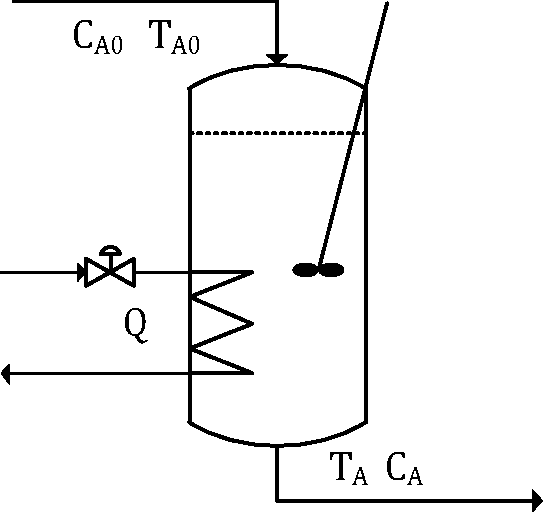
\includegraphics[scale=0.8]{cstr_diagram.pdf}
\caption{Diagram of a simple CSTR where the heat added to system is the only manipulated variable.}
\label{fig_cstr_diagram}
\end{figure}
The state space equations describing the reactor are shown in (\ref{eq_cstrmodel}) with parameters shown in Table \ref{tab_params}. The meaning of the variables is what one would expect from an intuitive understanding: $C_A$ is the concentration of species $A$, $T_R$ is the temperature of the CSTR and $Q$ is the heat added (or removed for negative $Q$) from the CSTR.
\begin{equation}
\begin{aligned}
\dot{C_A} &= \frac{F}{V}\left( C_{A0}-C_A \right) - k_0e^{\frac{-E}{RT_R}}C_A \\
\dot{T_R} &= \frac{F}{V}\left(T_{A0}-T_A\right) + \frac{-\triangle H}{\rho C_p}k_0e^{\frac{-E}{RT_R}}C_A + \frac{Q}{\rho C_p V}
\end{aligned}
\label{eq_cstrmodel}
\end{equation}
\begin{table}[H]
\begin{center}
\begin{tabular}{c c c c}
\hline
$V$ & $~0.1~m^3$ & $R$ & $~8.314~\frac{kJ}{kmol.K}$ \\
$C_{A0}$ & $~1.0~\frac{kmol}{m^3}$ &$T_{A0}$ & $~310~K$ \\
$\triangle H$ & $~-4.78\times 10^{4}~\frac{kJ}{kmol}$ & $k_{0}$ & $~72\times 10^{9}~\frac{1}{min}$ \\
$E$ & $~8.314\times 10^4~\frac{kJ}{kmol}$ & $C_{p}$ & $~0.239~\frac{kJ}{kg.K}$ \\
$\rho$ & $~1000~\frac{kg}{m^3}$ & 
$F$ & $~100\times 10^{-1}~\frac{m^3}{min}$ \\
\hline
\end{tabular}
\caption{CSTR parameters}
\label{tab_params}
\end{center}
\end{table}
The CSTR model is a familiar control example. Similar models may be found in \cite{du}\cite{cervantes}\cite{pan}\cite{yazdi}. We use this model because it is low dimensional yet complex enough to illustrate the principles we investigate.  

\subsection{Qualitative Analysis}
In this section we use standard mathematical tools, as found in \cite{edwardsandpenny}, to analyse the qualitative behaviour of the CSTR. By inspecting (\ref{eq_cstrmodel}) we see that the model is coupled and non-linear. By solving (\ref{eq_cstr_statpoints}) we see that for nominal operating conditions ($Q = 0$) there exist 3 operating points (critical points) as shown in Table \ref{tab_nominalstats}.
\begin{equation}
\begin{aligned}
0&= \frac{F}{V}\left( C_{A0}-C_A \right) - k_0e^{\frac{-E}{RT_R}}C_A \\
0 &= \frac{F}{V}\left(T_{A0}-T_A\right) + \frac{-\triangle H}{\rho C_p}k_0e^{\frac{-E}{RT_R}}C_A + \frac{Q}{\rho C_p V}
\end{aligned}
\label{eq_cstr_statpoints}
\end{equation}
\begin{table}[H]
\begin{center}
\begin{tabular}{c c c c}
\hline
Critical Point & $C_A$ & $T_R$ & Stability\\
\hline
$\left(C_A, T_R\right)_0^1$ & 0.0047 & 509.0604 & Stable Improper Node\\
$\left(C_A, T_R\right)_0^2$ & 0.5734 & 395.3268 & Unstable Saddle Point \\
$\left(C_A, T_R \right)_0^3$ & 0.9993 & 310.1429 & Stable Improper Node \\
\hline
\end{tabular}
\caption{Nominal operating points for  the CSTR}
\label{tab_nominalstats}
\end{center}
\end{table}
The stability of the operating points were found by linearising (\ref{eq_cstrmodel}) and computing the eigenvalues of the Jacobian, shown in (\ref{eq_jacobian}), at each critical point.
\begin{equation}
J(C_A, T_R) = \begin{pmatrix}
-\frac{F}{V} - k_0e^{\frac{-E}{RT_R}} & - k_0e^{\frac{-E}{RT_R}}C_A\left(\frac{E}{RT_R^2}\right) \\
\frac{-\triangle H}{\rho C_p}k_0e^{\frac{-E}{RT_R}} & -\frac{F}{V} + \frac{-\triangle H}{\rho C_p}k_0e^{\frac{-E}{RT_R}}C_A\left(\frac{E}{RT_R^2}\right) 
\end{pmatrix}
\label{eq_jacobian}
\end{equation}
In Figure \ref{fig_cstr_stat_points} we see how the stationary points move for $Q \in [-1272, 920]$\footnote{Q has units $\frac{kJ}{min}$}. It is clear that the stable operating points move in a relatively narrow range while the unstable operating point moves in a large range for different values of $Q$. Figure \ref{fig_cstr_stat_points} also indicates that clear regimes exist where, if one were to linearise (\ref{eq_cstrmodel}) about the critical points, linear approximations would be accurate.

Indeed, the approach of using piecewise affine (linear) functions for control, based on linearisation around critical points, has been investigated in literature \cite{du}\cite{kvasnica}. Typically the state domain is discretised into regimes and the linear approximation of the model in each regime is used for control. The benefit of this approach is that the non-linear problem  can then be handled by linear methods for which efficient algorithms exist. A potential drawback of this approach is computational complexity \cite{du}.
\begin{figure}[H] 
\centering
\includegraphics[scale=0.5]{cstr_model_stat_points.pdf}
\caption{CSTR stationary points as $Q$ changes. Each colour indicates the range of the associated operating point. Increasing values of Q monotonically increase the temperature component of each operating point.}
\label{fig_cstr_stat_points}
\end{figure}

\subsection{Linearised Models}
In this section we propose 3 linear models, each derived from the operating points of the CSTR under nominal conditions, to simplify the non-linear model. By using standard linearisation techniques the models in (\ref{eq_linearmodels}) are derived for each operating point, $i=1,2,3$, as found in Table \ref{tab_nominalstats}.
\begin{equation}
\dot{\begin{pmatrix}
C_A \\ T_R
\end{pmatrix}} \approx F\begin{pmatrix}
C_A \\ T_R \\ Q
\end{pmatrix}^i \equiv J(C_A, T_R)^i_0\begin{pmatrix}
C_A \\ T_R
\end{pmatrix} - J(C_A, T_R)^i_0\begin{pmatrix}
{C_A} \\ T_R
\end{pmatrix}_0^i + \begin{pmatrix}
0 \\ \frac{1}{\rho C_p V}
\end{pmatrix}Q
\label{eq_linearmodels}
\end{equation}
At this stage it is interesting to quantitatively evaluate the accuracy of each approximation. We use the Forward Euler finite difference scheme to discretise (\ref{eq_linearmodels}) as shown in (\ref{eq_discretemodels}). While the Forward Euler method is only conditionally stable, and hence convergent because the system is linear, it is easy to apply and the resultant models are of a form amenable to our purposes in later sections. The drawback of using Forward Euler is that a small time step, $h$, must be used.
\begin{equation}
\begin{pmatrix}
C_A \\ T_R
\end{pmatrix}_{t+1} \approx  \begin{pmatrix}
C_A \\ T_R
\end{pmatrix}_{t} + h F\begin{pmatrix}
C_A \\ T_R \\ Q 
\end{pmatrix}_t^i
\label{eq_discretemodels}
\end{equation}
In Figures \ref{fig_cstr_op1} to \ref{fig_cstr_op3} we see the transient\footnote{The time step is set at $h=0.001$.}, unforced\footnote{That is $Q=0$}, response of the linearised systems with different initial conditions. The non-linear system is also shown to compare the accuracy of the linearisation. Each initial condition was chosen to be close to an operating point and the time scales were adjusted for clarity. 
\begin{figure}[H] 
\centering
\includegraphics[scale=0.40]{cstr_op1.pdf}
\caption{Unforced transient response of the CSTR with initial condition $C_A = 0.05,T_R=520$.}
\label{fig_cstr_op1}
\end{figure}
\begin{figure}[H] 
\centering
\includegraphics[scale=0.40]{cstr_op2.pdf}
\caption{Unforced transient response of the CSTR with initial condition $C_A = 0.57,T_R=395$.}
\label{fig_cstr_op2}
\end{figure}
\begin{figure}[H] 
\centering
\includegraphics[scale=0.40]{cstr_op3.pdf}
\caption{Unforced transient response of the CSTR with initial condition $C_A = 0.9,T_R=350$.}
\label{fig_cstr_op3}
\end{figure}
From the figures above it is clear, and also not surprising, that the linear models are most accurate if the trajectory of the states $C_A$ and $T_R$ is near the point of linearisation. From this one may conclude that if a linear model must be used to control the CSTR, it is better to use a linear model which was linearised close to the current trajectory.

It is desirable to attempt to make precise what we mean by ``was linearised close to the current trajectory" as stated in the previous paragraph. If this is possible it would be easy to decide which linear model to use based on the current state estimate or prediction.

Consider Figure \ref{fig_cstr_op4} which shows the unforced response of the CSTR from an initial condition which is closer, in the sense of the Euclidean norm, to the unstable operating point $(C_A, T_R)_0^2$. It is clear that initially the linear model linearised around unstable operating point $(C_A, T_R)_0^2$ best describes the reactor dynamics. As time progresses the system moves toward the stable $(C_A, T_R)_0^1$ operating point and the associated linear model becomes better. Intuitively this is what one would expect based on Figures \ref{fig_cstr_op1} to \ref{fig_cstr_op3}.
\begin{figure}[H] 
\centering
\includegraphics[scale=0.4]{cstr_op4.pdf}
\caption{Unforced transient response of the CSTR with initial condition $C_A = 0.5,T_R=410$.}
\label{fig_cstr_op4}
\end{figure}
Now we attempt predict the Euclidean error of the state vector based on the Euclidean distance from the linearisation point. In Figure \ref{fig_cstr_op5} we see that during all but the short initial period ($t \in [0, 0.01]$) the linear model linearised around $(C_A, T_R)_0^1$ is closer to its operating point than the linear model linearised around the unstable operating point $(C_A, T_R)_0^2$. Unfortunately the Euclidean error does not follow this trend. We see that even though the linear model $(C_A, T_R)_0^2$ is further away it is a better model until $t \approx 0.2$.  
\begin{figure}[H] 
\centering
\includegraphics[scale=0.4]{cstr_op5.pdf}
\caption{Euclidean distance for each linear model from the linearisation point. Euclidean error for each model from the non-linear trajectory.}
\label{fig_cstr_op5}
\end{figure}
This problem is general in nature: it is better (and easier) to choose which model to use based on the observed difference between the actual system and the set of possible linear models. It is also easy to hypothesise that using more linear models is better than using less. In our example we used 3 because there were 3 operating points, but there is no theoretical reason why one cannot linearise a system about an arbitrary point in the state space.

Thus, if it is desirable to use a set of linear models for control we require a systematic method to infer which model best describes the system based on the current observation. Ideally the control policy should then be based upon this model. If we add measurement noise and plant uncertainty into the equation it becomes clear that advanced methods will be required. 

%\bibliographystyle{plain}
%\bibliography{research}

\end{document}